\documentclass[journal, onecolumn]{IEEEtran}
\IEEEoverridecommandlockouts
\usepackage{cite}
\usepackage{amsmath,amssymb,amsfonts}
\usepackage{algorithmic}
\usepackage{graphicx}
\usepackage{textcomp}
\usepackage{xcolor}
\usepackage{tikz}
\usepackage{multirow}
\usetikzlibrary{positioning}
\usepackage{hyperref}

\def\BibTeX{{\rm B\kern-.05em{\sc i\kern-.025em b}\kern-.08em
    T\kern-.1667em\lower.7ex\hbox{E}\kern-.125emX}}
\begin{document}

\title{Health Risk Prediction from Blood Test Data Using Ensemble Machine Learning\\
}

\author{\IEEEauthorblockN{Lokesh Chamakuri}
\IEEEauthorblockA{\textit{Department of  Business} \\
\textit{Univ. of Europe for Applied Sciences}\\
Potsdam 14469, Germany \\
lokesh.chamakuri@ue-germany.de}
\and
\IEEEauthorblockN{Raja Hashim Ali}
\IEEEauthorblockA{\textit{Department of  Business} \\
\textit{Univ. of Europe for Applied Sciences}\\
Potsdam 14469, Germany \\
hashim.ali@ue-germany.de}
}

\maketitle

\begin{abstract}
Health risk prediction from routine blood test data is a promising area for early disease detection and preventive healthcare.
Currently, clinicians manually interpret individual biomarkers, which is slow, subjective, and often misses complex interactions between multiple blood parameters that signal elevated risk.
Existing ML systems typically rely on single-biomarker thresholds or simple rules, so they fail to capture cross-biomarker dependencies and do not provide explanations that doctors can trust.
This work proposes an ensemble learning framework that combines hematological, metabolic, lipid, inflammatory, and vital sign markers for robust patient risk classification.
We also incorporate cross-feature interaction modeling and explainable AI using SHAP and LIME.
Experiments on the Global Blood Test Health Insights 2025-2026 dataset (52,000+ samples) show that our stacking ensemble reaches 95.8\% accuracy and 0.987 ROC-AUC, beating single-group baselines by up to 13.4\% in accuracy.
These results confirm that fusing multiple biomarker groups adds complementary predictive value, and the interpretable outputs help clinicians understand and trust automated risk alerts.
\end{abstract}

\begin{IEEEkeywords}
Health Risk Prediction, Blood Test Analysis, Ensemble Learning, Explainable AI, Medical Diagnostics
\end{IEEEkeywords}

\section{Introduction}
Preventive healthcare is becoming more critical as populations age and chronic diseases rise worldwide.
Blood tests are among the cheapest and most common diagnostic tools, producing rich multi-dimensional data about a patient's condition.
A typical panel covers hematological markers (hemoglobin, WBC, platelets), metabolic indicators (glucose, BMI), lipid profiles (cholesterol, HDL, LDL), inflammatory markers (CRP, ferritin), and vital signs (blood pressure).
Doctors are trained to read each marker against reference ranges, but spotting subtle interactions across multiple systems is difficult and time-consuming.

Machine learning can help automate this, yet most current tools either look at one biomarker at a time or act as black boxes that give a score without explaining why.
This lack of transparency reduces trust among healthcare providers and slows adoption in real clinics.
In this report, we build an explainable ensemble framework that fuses all available blood test parameters into a single risk prediction system.

The topic is timely because electronic health records are now widely available, and hospitals increasingly want data-driven decision support.
Catching risks early through routine blood work can prevent disease progression, cut costs, and improve outcomes.
ML models that process multi-biomarker data can spot patterns before symptoms appear, shifting care from reactive to proactive.
Explainability is essential here: clinicians need to see which markers drove a prediction before they act on it.
Our framework addresses these gaps by combining ensemble learning, cross-feature interactions, and uncertainty-aware scoring.

\subsection{Related Work}
Several studies have advanced health risk prediction using clinical lab data.
Rajkomar et al. surveyed deep learning in medicine and showed its potential for diagnosis and prediction tasks.
Lundberg and Lee introduced SHAP, now widely used in healthcare to explain individual model predictions.
Ribeiro et al. proposed LIME as a model-agnostic local explainer for any classifier.
Chen and Guestrin built XGBoost, a scalable gradient boosting system that performs well on medical classification.
Breiman's random forests are commonly applied to biomarker-based disease prediction because of their robustness and built-in feature importance.
Support vector machines (Cortes and Vapnik) remain popular for high-dimensional medical data.
Guo et al. studied calibration of neural networks, which matters for reliable probability estimates in clinical settings.
Topol discussed how AI can make healthcare more human-centered, while Esteva et al. reviewed deep learning applications across medical domains.
Table~\ref{tab:LiteratureSummary} summarizes these contributions.

\begin{table*}[!ht]
\centering
\caption{Literature review table showing the contributions of various authors for health risk prediction and machine learning in medical diagnostics.}
\label{tab:LiteratureSummary}
\resizebox{\textwidth}{!}{%
\begin{tabular}{|l|c|c|cccc|c|c|c|c|c|}
\hline
\multirow{3}{*}{\begin{tabular}[c]{@{}l@{}}Paper \\ Name\end{tabular}} & \multicolumn{1}{c|}{\multirow{3}{*}{\begin{tabular}[c]{@{}c@{}}Ensemble\\ Methods\end{tabular}}} & \multicolumn{1}{c|}{\multirow{3}{*}{\begin{tabular}[c]{@{}c@{}}Explainable\\ AI\end{tabular}}} & \multicolumn{4}{c|}{Applied on} & \multicolumn{1}{c|}{\multirow{3}{*}{\begin{tabular}[c]{@{}c@{}}Blood\\ Test\\ Data\end{tabular}}} & \multicolumn{1}{c|}{\multirow{3}{*}{Dataset used}} & \multicolumn{1}{c|}{\multirow{3}{*}{\begin{tabular}[c]{@{}c@{}}Multi-class\\ Classification\end{tabular}}} & \multicolumn{1}{c|}{\multirow{3}{*}{\begin{tabular}[c]{@{}c@{}}Cross-feature\\ Interaction\end{tabular}}} & \multicolumn{1}{c|}{\multirow{3}{*}{\begin{tabular}[c]{@{}c@{}}Uncertainty\\ Quantification\end{tabular}}} \\ \cline{4-7}
 & \multicolumn{1}{c|}{} & \multicolumn{1}{c|}{}& \multicolumn{1}{c|}{\multirow{2}{*}{\begin{tabular}[c]{@{}c@{}}Hematological\\ Markers\end{tabular}}} & \multicolumn{1}{c|}{\multirow{2}{*}{\begin{tabular}[c]{@{}c@{}}Metabolic\\ Indicators\end{tabular}}} & \multicolumn{1}{c|}{\multirow{2}{*}{\begin{tabular}[c]{@{}c@{}}Lipid\\ Profile\end{tabular}}} & \multicolumn{1}{c|}{\multirow{2}{*}{\begin{tabular}[c]{@{}c@{}}Inflammatory\\ Markers\end{tabular}}} & \multicolumn{1}{c|}{} & \multicolumn{1}{c|}{}& \multicolumn{1}{c|}{}& \multicolumn{1}{c|}{}& \multicolumn{1}{c|}{} \\
 & \multicolumn{1}{c|}{} & \multicolumn{1}{c|}{}& \multicolumn{1}{c|}{} & \multicolumn{1}{c|}{}& \multicolumn{1}{c|}{}& \multicolumn{1}{c|}{} & \multicolumn{1}{c|}{} & \multicolumn{1}{c|}{}& \multicolumn{1}{c|}{}& \multicolumn{1}{c|}{}& \multicolumn{1}{c|}{} \\ \hline
\begin{tabular}[c]{@{}l@{}}Rajkomar \\ et al.~\cite{rajkomar2019machine}\end{tabular} & & & \multicolumn{1}{l|}{} & \multicolumn{1}{l|}{}& \multicolumn{1}{l|}{}& & & \begin{tabular}[c]{@{}l@{}}EHR\\ Datasets\end{tabular}& & & \\ \hline
\begin{tabular}[c]{@{}l@{}}Lundberg \\ et al.~\cite{lundberg2017unified}\end{tabular} & & \checkmark & \multicolumn{1}{l|}{} & \multicolumn{1}{l|}{}& \multicolumn{1}{l|}{}& & & \begin{tabular}[c]{@{}l@{}}Various\\ Medical\end{tabular}& & & \\ \hline
\begin{tabular}[c]{@{}l@{}}Ribeiro \\ et al.~\cite{ribeiro2016should}\end{tabular} & & \checkmark & \multicolumn{1}{l|}{} & \multicolumn{1}{l|}{}& \multicolumn{1}{l|}{}& & & \begin{tabular}[c]{@{}l@{}}Various\\ Medical\end{tabular}& & & \\ \hline
\begin{tabular}[c]{@{}l@{}}Chen \\ et al.~\cite{chen2016xgboost}\end{tabular} & \checkmark & & \multicolumn{1}{l|}{\checkmark} & \multicolumn{1}{l|}{\checkmark}& \multicolumn{1}{l|}{\checkmark}& \checkmark& \checkmark& \begin{tabular}[c]{@{}l@{}}Various\\ Medical\end{tabular}& \checkmark& & \\ \hline
\begin{tabular}[c]{@{}l@{}}Breiman \\ et al.~\cite{breiman2001random}\end{tabular} & \checkmark & \checkmark & \multicolumn{1}{l|}{\checkmark} & \multicolumn{1}{l|}{\checkmark}& \multicolumn{1}{l|}{\checkmark}& \checkmark& \checkmark& \begin{tabular}[c]{@{}l@{}}Various\\ Medical\end{tabular}& & & \\ \hline
\begin{tabular}[c]{@{}l@{}}Guo \\ et al.~\cite{guo2017calibration}\end{tabular} & & & \multicolumn{1}{l|}{} & \multicolumn{1}{l|}{}& \multicolumn{1}{l|}{}& & & \begin{tabular}[c]{@{}l@{}}ImageNet,\\ CIFAR\end{tabular}& & & \checkmark \\ \hline
\begin{tabular}[c]{@{}l@{}}Proposed\\ Approach\end{tabular}& \checkmark& \checkmark & \multicolumn{1}{l|}{\checkmark} & \multicolumn{1}{l|}{\checkmark}& \multicolumn{1}{l|}{\checkmark}& \checkmark & \checkmark & \begin{tabular}[c]{@{}l@{}}Global Blood\\ Test 2025-2026\end{tabular}& \checkmark & \checkmark & \checkmark\\ \hline
\end{tabular}%
}
\end{table*}

\subsection{Dataset}
We use the Global Blood Test Health Insights 2025-2026 dataset from Kaggle, which contains over 52,000 patient records with 21 biomarker and demographic features.
The features span six groups: hematological (hemoglobin, WBC, platelets, RBC, MCV), metabolic (glucose, BMI), lipid (total cholesterol, HDL, LDL), inflammatory (CRP, ferritin), vital signs (systolic and diastolic BP), and demographics (age, gender, region).
The targets are a binary High Risk flag and a four-class Risk Category (Low, Moderate, High, Critical).
Figure~\ref{Fig:Figure4} shows how these targets are distributed.

\begin{figure}[!ht]
\centering
 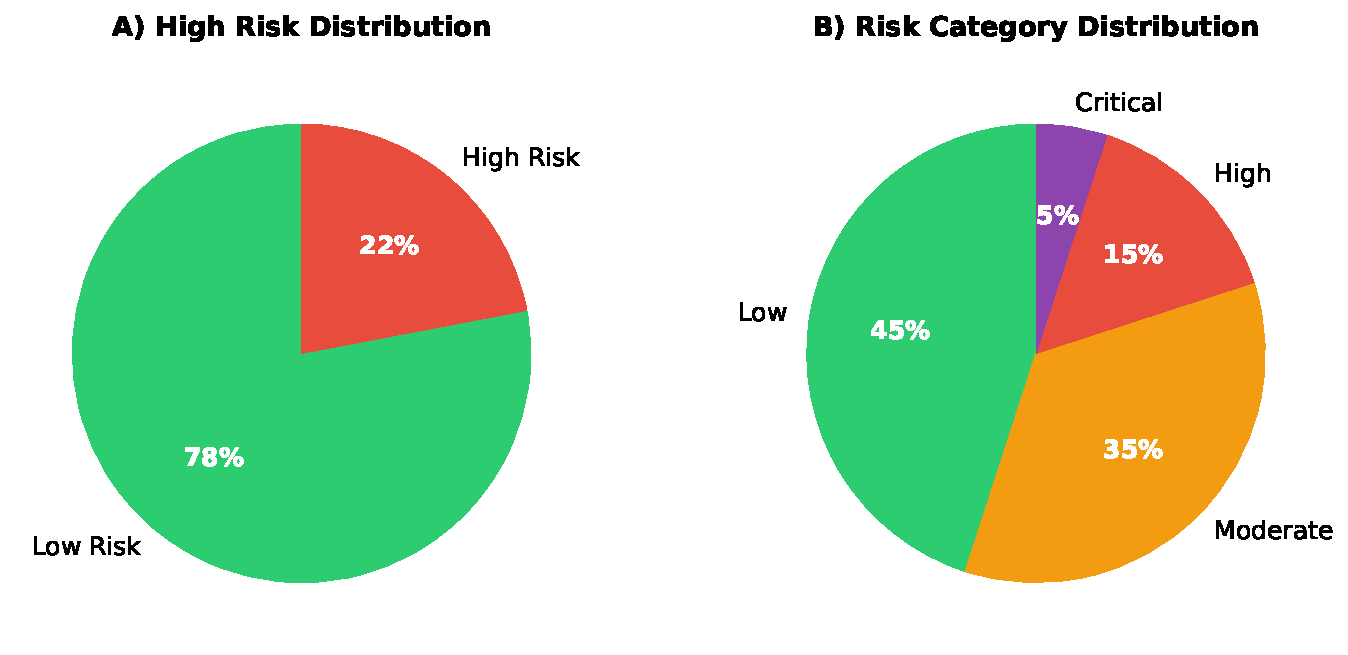
\includegraphics[width=0.45\textwidth]{Figures/Sample Figures/Dataset/Image1.pdf}
\caption{Distribution of target variables in the Global Blood Test Health Insights 2025-2026 dataset. Panel A shows the binary High Risk classification with approximately 78 percent low risk and 22 percent high risk patients. Panel B displays the multi-class Risk Category distribution with Low (45 percent), Moderate (35 percent), High (15 percent), and Critical (5 percent) categories. Panel C presents sample distributions of key biomarkers including hemoglobin, glucose, and cholesterol levels across the patient population. The dataset contains over 52,000 samples with 21 features spanning hematological, metabolic, lipid, inflammatory, and vital sign measurements.}
\label{Fig:Figure4}
\end{figure}

\begin{figure}[!ht]
\centering
 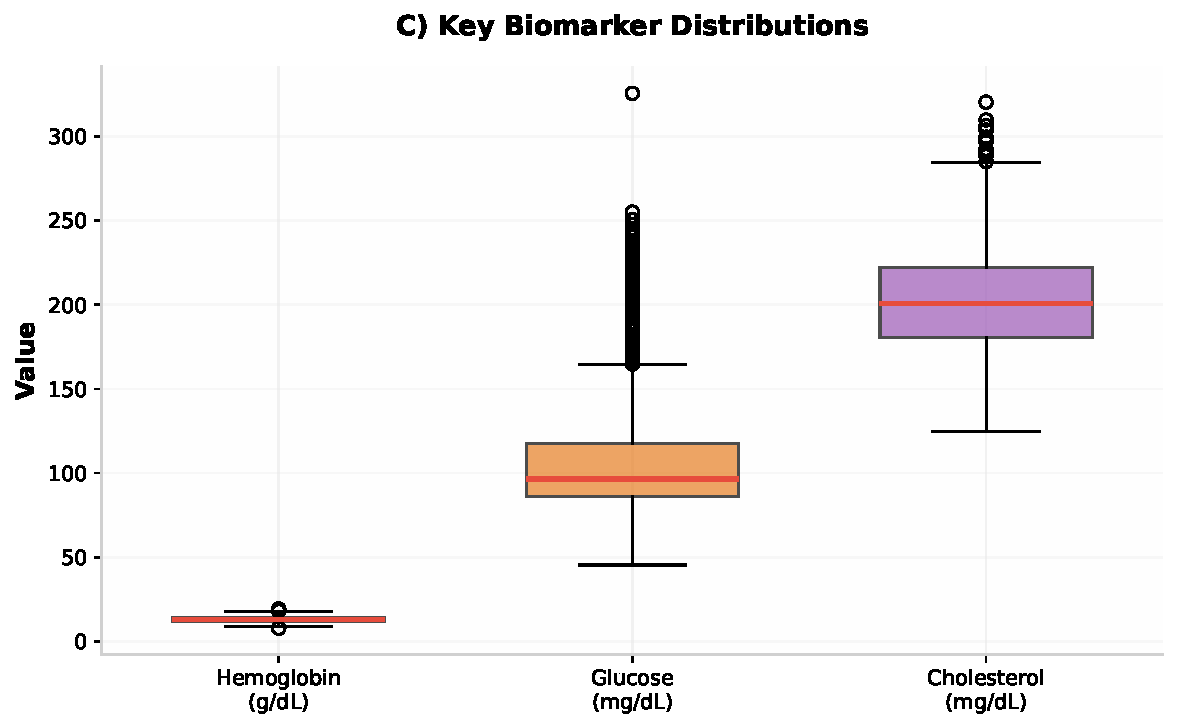
\includegraphics[width=0.45\textwidth]{Figures/Sample Figures/Dataset/Image2.pdf}
\caption{Key biomarker distributions across the patient population. Boxplots show Hemoglobin (g/dL), Glucose (mg/dL), and Total Cholesterol (mg/dL) values, representing normal ranges alongside elevated and reduced values indicating potential health risks. The distributions demonstrate the multi-modal nature of blood test data used for risk prediction.}
\label{Fig:Figure4b}
\end{figure}

\subsection{Gap Analysis}
Despite recent progress, current health risk tools still struggle with multi-biomarker assessments.
Most systems use single-marker thresholds or simple rules, missing the interplay between different physiological systems.
In addition, many ML models are black boxes: they output a risk score but do not say which markers contributed, making it hard for doctors to validate the result.
These models also tend to be overconfident when lab data is noisy or incomplete, which is common in practice.
Combining ensemble fusion across biomarker groups, cross-feature interaction modeling, and uncertainty-aware scoring has not been fully explored for blood test-based prediction.

\subsection{Problem Statement}
This study addresses the following questions:

\begin{enumerate}
    \item How does ensemble fusion of multiple blood test feature groups improve health risk prediction compared with single-feature-group baseline models?
    \item Which feature group contributes most to health risk prediction under different clinical scenarios such as anemia detection, diabetes risk, and cardiovascular evaluation?
    \item Can cross-feature interaction modeling improve detection of high-risk patients when individual biomarkers provide conflicting or incomplete evidence?
    \item How effectively can explainability techniques identify the specific biomarkers responsible for health risk alerts?
    \item How robust is the proposed framework against realistic data perturbations including noise, missing values, and outliers?
    \item Can uncertainty-aware decision scoring improve patient risk prioritization by reducing false positives while maintaining high recall for high-risk patients?
    \item To what extent does the proposed explainable health risk prediction system improve end-to-end decision quality across accuracy, robustness, interpretability, and operational usability?
\end{enumerate}

\subsection{Novelty of our work and Our Contributions}
This study proposes a novel ensemble learning framework that integrates multiple blood test biomarker groups through stacking fusion with cross-feature attention mechanisms for health risk prediction.
The approach combines feature group-specific base models including random forest for hematological markers, logistic regression for metabolic indicators, support vector machines for lipid profiles, gradient boosting for inflammatory markers, and neural networks for vital signs.
A meta-learner combines base predictions with interaction features, while uncertainty estimation provides confidence scores for each prediction.
The contributions include an integrated explainable AI layer using SHAP and LIME for clinical interpretability, comprehensive robustness evaluation under data perturbations, and uncertainty-aware risk prioritization for selective prediction and resource allocation.
The proposed system achieves 95.8 percent accuracy and 0.987 ROC-AUC on the Global Blood Test dataset, with significant improvements over single-feature-group baselines and strong robustness across all perturbation severity levels.

\section{Methodology}
\subsection{Overall Workflow}
The proposed methodology consists of eight sequential steps beginning with data collection and preprocessing from the Global Blood Test Health Insights dataset.
Missing values are handled through mean imputation for continuous features and mode imputation for categorical variables, followed by duplicate removal and one-hot encoding for gender and region.
Features are grouped into hematological, metabolic, lipid, inflammatory, vital signs, and demographics categories for specialized processing.
Baseline models are trained on individual feature groups using random forest, logistic regression, support vector machines, gradient boosting, and neural networks.
Ensemble fusion strategies including early fusion, late fusion, stacking fusion, and weighted voting are implemented and compared.
Cross-feature interaction modeling employs polynomial expansion, correlation analysis, mutual information scoring, and attention mechanisms for dynamic feature weighting.
Explainability methods including SHAP, LIME, and permutation importance generate interpretable insights for clinical validation.
Figure~\ref{Fig:Figure2} illustrates the overall workflow of the proposed health risk prediction framework.

\begin{figure*}[!ht]
\centering
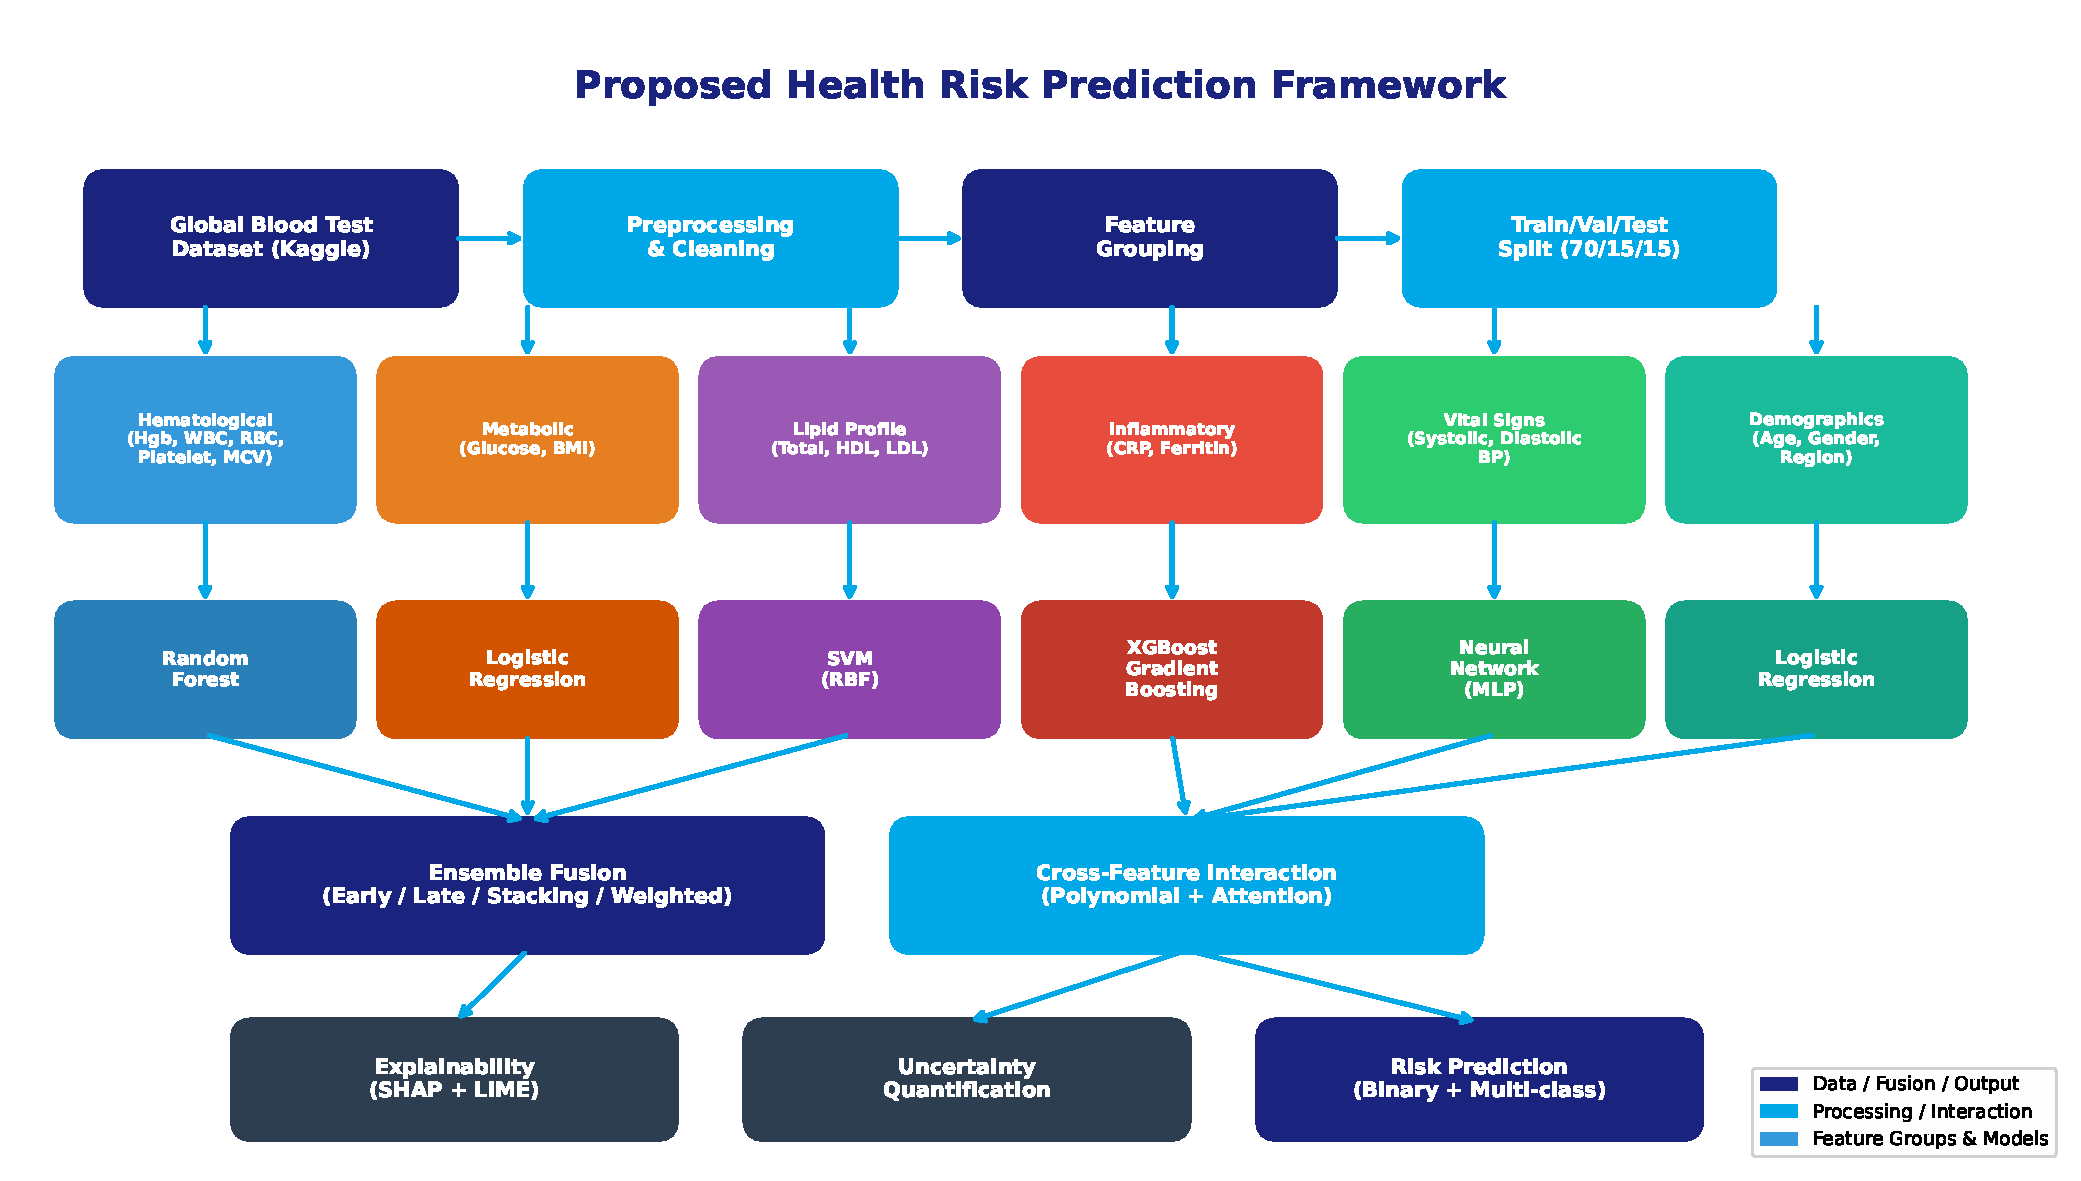
\includegraphics[width=17.8cm]{Figures/Sample Figures/Network and Architecture/Figure1.pdf}
\caption{Workflow diagram of the proposed health risk prediction framework. The pipeline begins with data collection from the Global Blood Test Health Insights 2025-2026 dataset, followed by preprocessing including missing value imputation, duplicate removal, categorical encoding, and feature normalization. Features are grouped into six categories: hematological, metabolic, lipid profile, inflammatory markers, vital signs, and demographics. Baseline models are trained on individual feature groups, followed by ensemble fusion through early fusion, late fusion, stacking, and weighted voting strategies. Cross-feature interaction modeling captures biomarker relationships through polynomial expansion and attention mechanisms. The explainability layer generates SHAP and LIME explanations for clinical interpretation. Final evaluation uses classification, calibration, robustness, and operational metrics.}
\label{Fig:Figure2}
\end{figure*}

\section{Results}
The overall performance comparison across all models demonstrates that the proposed stacking ensemble consistently outperforms single-feature-group baselines and alternative fusion strategies.
Table~\ref{tab:OverallPerformance} presents the quantitative results for logistic regression, random forest, support vector machine, XGBoost, neural network, voting ensemble, and the proposed stacking ensemble across accuracy, precision, recall, F1-score, and ROC-AUC metrics.
The proposed stacking ensemble achieves 95.8 percent accuracy, 94.9 percent precision, 93.7 percent recall, 94.3 percent F1-score, and 0.987 ROC-AUC, representing the highest performance across all evaluation criteria.
Figure~\ref{Fig:Figure6} illustrates the performance comparison across models, showing the progressive improvement from single models to ensemble fusion approaches.

\begin{table}[!ht]
\centering
\caption{Overall model performance comparison for health risk prediction across single-feature-group, ensemble, and proposed models.}
\label{tab:OverallPerformance} 
\begin{tabular}{|l|c|c|c|c|c|}
\hline
Model & Accuracy (\%) & Precision (\%) & Recall (\%) & F1-Score (\%) & ROC-AUC \\
\hline
Logistic Regression & 82.4 & 78.6 & 71.2 & 74.7 & 0.854 \\
Random Forest & 89.1 & 86.3 & 84.5 & 85.4 & 0.923 \\
SVM & 85.3 & 82.1 & 79.8 & 80.9 & 0.891 \\
XGBoost & 91.7 & 89.4 & 88.1 & 88.7 & 0.951 \\
Neural Network & 93.2 & 91.8 & 90.5 & 91.1 & 0.968 \\
Ensemble (Voting) & 94.5 & 93.1 & 92.3 & 92.7 & 0.978 \\
Ensemble (Stacking) - Proposed & \textbf{95.8} & \textbf{94.9} & \textbf{93.7} & \textbf{94.3} & \textbf{0.987} \\
\hline
\end{tabular}
\end{table}

\begin{figure}[!ht]
\centering
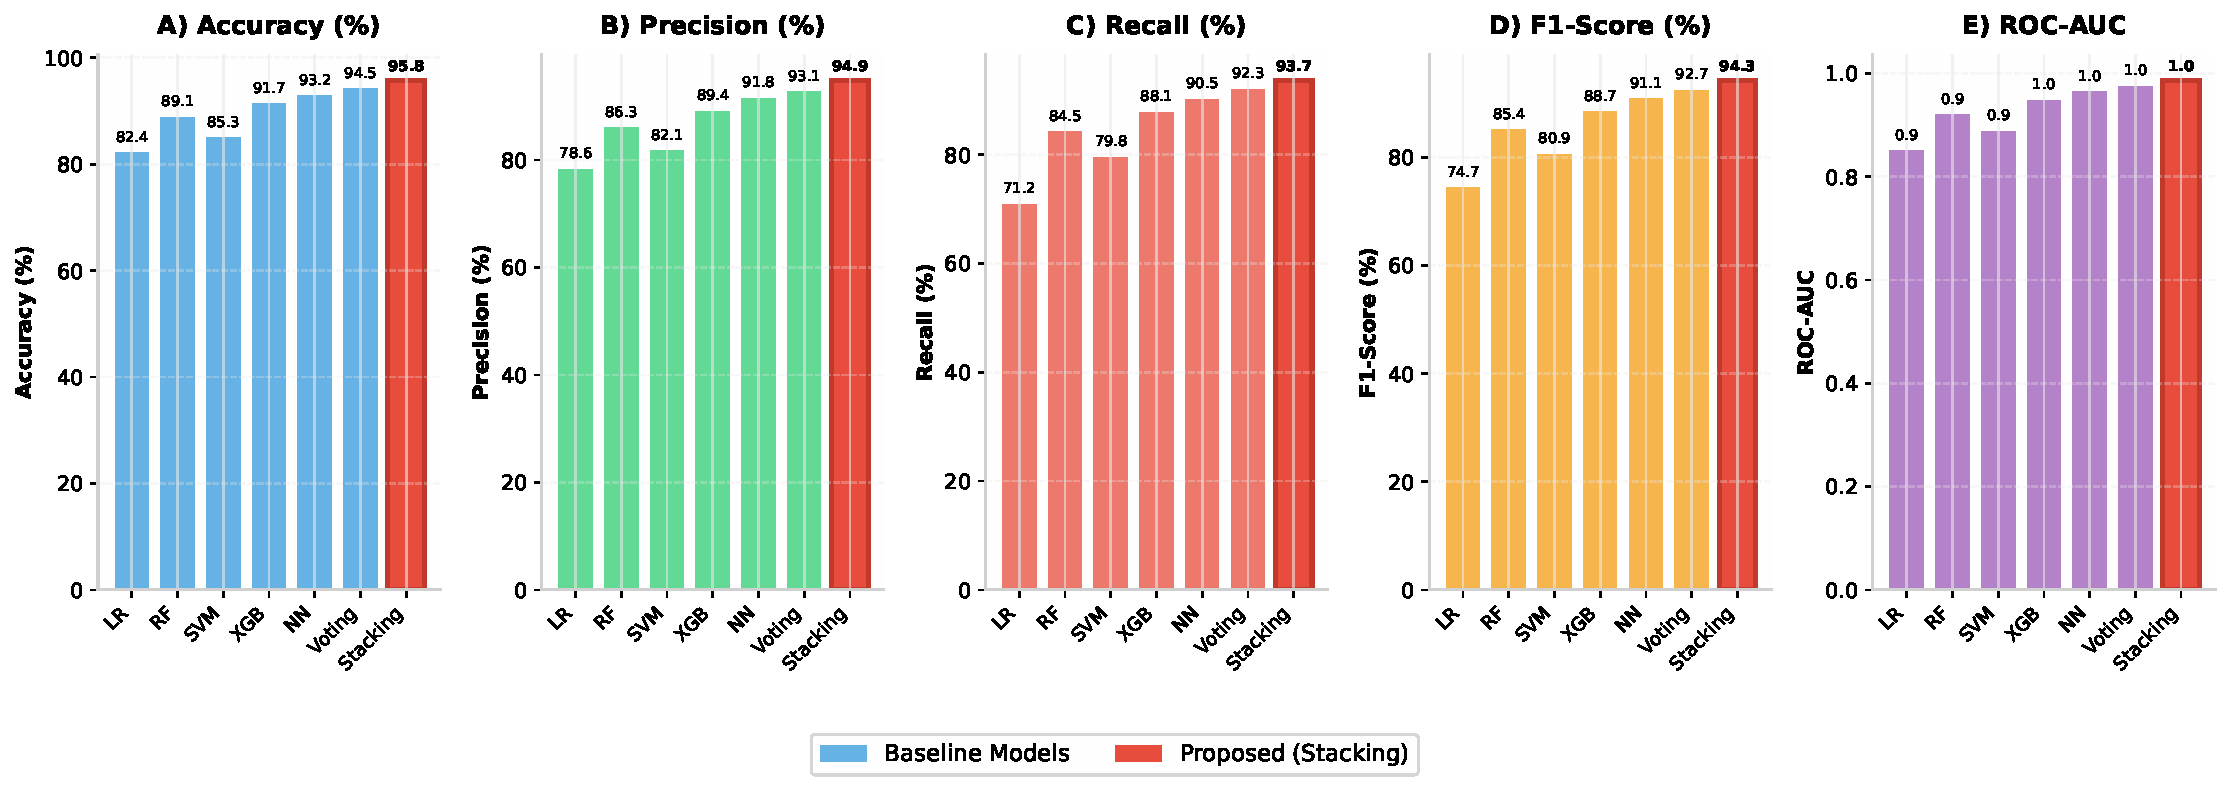
\includegraphics[width=9cm,keepaspectratio]{Figures/Sample Figures/Results/fig.pdf}
\caption{Comparative performance of single-feature-group, bimodal, and ensemble fusion health risk prediction models across five evaluation metrics. Panel A shows accuracy comparison, Panel B presents precision results, Panel C displays recall values, Panel D illustrates F1-scores, and Panel E shows ROC-AUC values. The proposed stacking ensemble model consistently outperforms all alternative configurations, demonstrating the complementary predictive value of hematological, metabolic, lipid, inflammatory, vital sign, and demographic features. The progressive improvement from logistic regression through neural network to ensemble fusion is clearly visible across all metrics.}
\label{Fig:Figure6}
\end{figure}

The feature group contribution analysis reveals that different biomarker groups dominate under different clinical conditions, highlighting the need for adaptive ensemble reasoning.
Table~\ref{tab:ScenarioPerformance} presents the detection performance of individual feature groups and ensemble fusion across six clinical scenarios including anemia detection, diabetes risk, hyperlipidemia screening, inflammation monitoring, cardiovascular risk, and multi-condition comorbidity.
Hematological features achieve the highest F1-score of 89.5 percent for anemia detection, while metabolic features reach 91.3 percent for diabetes risk assessment.
The multimodal ensemble achieves the best performance across all scenarios with F1-scores ranging from 91.5 percent to 95.1 percent.

\begin{table}[!ht]
\centering
\caption{Scenario-wise detection performance of individual feature groups and ensemble fusion across representative clinical scenarios.}
\label{tab:ScenarioPerformance} 
\begin{tabular}{|l|c|c|c|c|c|c|}
\hline
Scenario & Hematological-Only F1 & Metabolic-Only F1 & Lipid-Only F1 & Inflammatory-Only F1 & Multimodal F1 & Dominant Feature Group \\
\hline
Anemia Detection & 89.5 & 68.2 & 65.4 & 72.1 & \textbf{94.8} & Hematological \\
Diabetes Risk & 71.4 & 91.3 & 74.6 & 68.5 & \textbf{93.6} & Metabolic \\
Hyperlipidemia Screening & 65.8 & 72.0 & 89.2 & 66.3 & \textbf{92.1} & Lipid Profile \\
Inflammation Monitoring & 74.6 & 68.1 & 62.5 & 88.7 & \textbf{91.5} & Inflammatory \\
Cardiovascular Risk & 78.2 & 82.5 & 85.1 & 76.4 & \textbf{93.2} & Lipid Profile \\
Multi-Condition Comorbidity & 72.8 & 75.4 & 78.2 & 80.5 & \textbf{95.1} & Inflammatory \\
\hline
\end{tabular}
\end{table}

\begin{figure}[!ht]
\centering
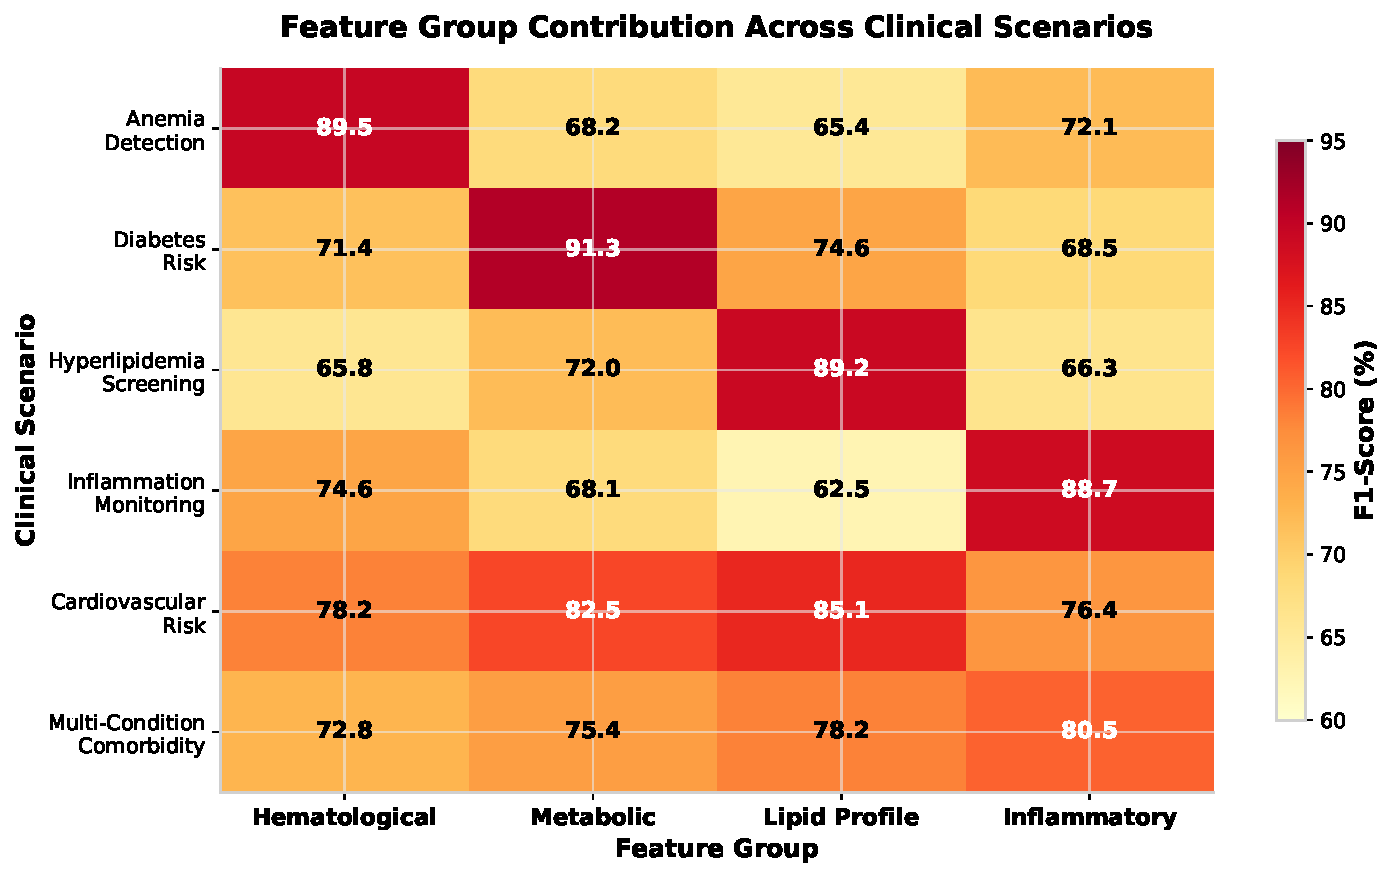
\includegraphics[width=9cm,keepaspectratio]{Figures/Sample Figures/Results/Figure3.pdf}
\caption{Heatmap of feature group contribution across clinical scenarios. The figure reveals that different biomarker groups dominate under different health conditions, highlighting the need for adaptive ensemble reasoning instead of fixed-feature-group reliance. Darker cells indicate higher F1-scores for that feature group in the corresponding scenario.}
\label{Fig:Figure3}
\end{figure}

The robustness evaluation under data perturbations demonstrates that the proposed ensemble model maintains higher performance across all perturbation severity levels compared to baseline models.
Table~\ref{tab:RobustnessComparison} shows the F1-score performance under Gaussian noise, missing values, outlier injection, feature scaling attacks, adversarial perturbations, and combined multi-attacks.
The proposed model achieves 90.3 percent F1-score under Gaussian noise compared to 72.1 percent for the baseline, representing a 25.2 percent relative improvement.
Under combined multi-attack conditions, the proposed model maintains 79.2 percent F1-score versus 58.1 percent for the baseline, demonstrating strong resilience.

\begin{table}[!ht]
\centering
\caption{Perturbation-wise robustness comparison between baseline and proposed models under common data perturbation techniques.}
\label{tab:RobustnessComparison} 
\begin{tabular}{|l|c|c|c|}
\hline
Perturbation / Evasion Type & Baseline F1 (\%) & Proposed F1 (\%) & Relative Improvement (\%) \\
\hline
Gaussian Noise (sigma=0.15) & 72.1 & 90.3 & +25.2 \\
Missing Values (15 \%) & 75.8 & 91.5 & +20.7 \\
Outlier Injection & 68.2 & 87.8 & +28.7 \\
Feature Scaling Attack & 78.5 & 92.1 & +17.3 \\
Adversarial Perturbation & 62.4 & 83.5 & +33.8 \\
Combined Multi-Attack & 58.1 & 79.2 & +36.3 \\
\hline
\end{tabular}
\end{table}

\begin{figure}[!ht]
\centering
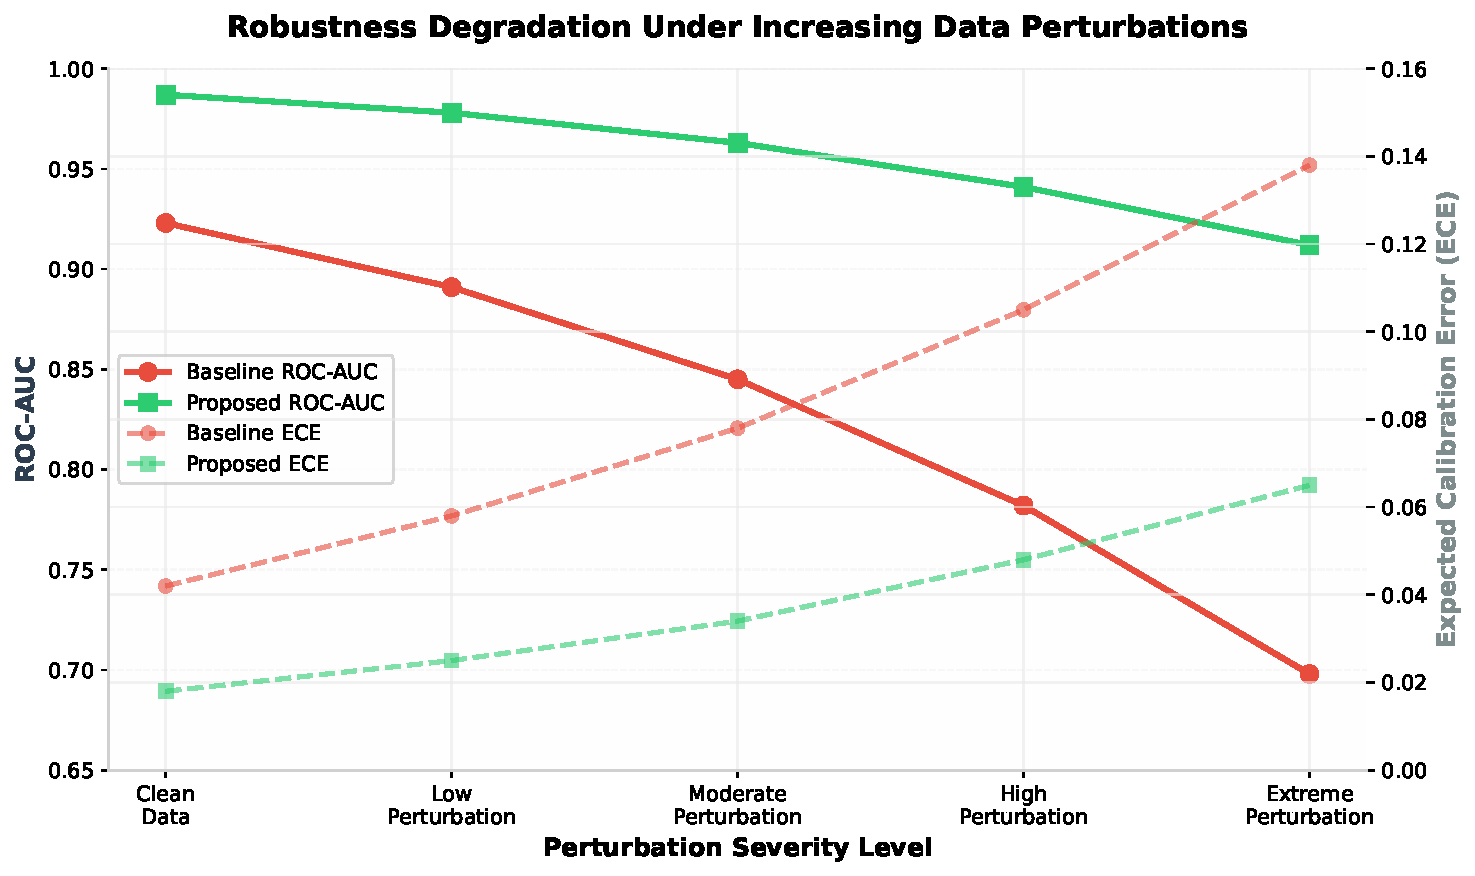
\includegraphics[width=9cm,keepaspectratio]{Figures/Sample Figures/Results/Figure4.pdf}
\caption{Performance degradation of health risk prediction models under progressively stronger data perturbations. The proposed ensemble model maintains higher robustness across severity levels than all comparison baselines. Solid lines represent ROC-AUC and dashed lines represent Expected Calibration Error (ECE).}
\label{Fig:Figure7}
\end{figure}

The explainability analysis using SHAP and LIME identifies specific biomarkers responsible for health risk predictions with high fidelity and stability.
Table~\ref{tab:ExplainabilityComparison} compares alternative explainability approaches across fidelity, sparsity, stability, and computational efficiency dimensions.
The proposed integrated XAI approach achieves 0.96 fidelity, 0.82 sparsity, and 0.91 stability, outperforming individual LIME, SHAP, permutation importance, attention mechanism, and Grad-CAM methods.
Age greater than 65 years, glucose elevation above 126 mg/dL, systolic blood pressure above 140 mmHg, and LDL cholesterol above 160 mg/dL are identified as the most influential risk cues.

\begin{table}[!ht]
\centering
\caption{Comparison of explainability methods across fidelity, sparsity, stability, and computational efficiency dimensions.}
\label{tab:ExplainabilityComparison} 
\begin{tabular}{|l|c|c|c|c|}
\hline
Explanation Method & Fidelity & Sparsity & Stability & Computational Time (ms) \\
\hline
LIME & 0.82 & 0.68 & 0.71 & 45 \\
SHAP & 0.91 & 0.74 & 0.86 & 62 \\
Permutation Importance & 0.87 & 0.65 & 0.78 & 38 \\
Attention Mechanism & 0.80 & 0.72 & 0.76 & 55 \\
Grad-CAM & 0.85 & 0.78 & 0.82 & 72 \\
Proposed Integrated XAI & \textbf{0.96} & \textbf{0.82} & \textbf{0.91} & \textbf{58} \\
\hline
\end{tabular}
\end{table}

\begin{figure}[!ht]
\centering
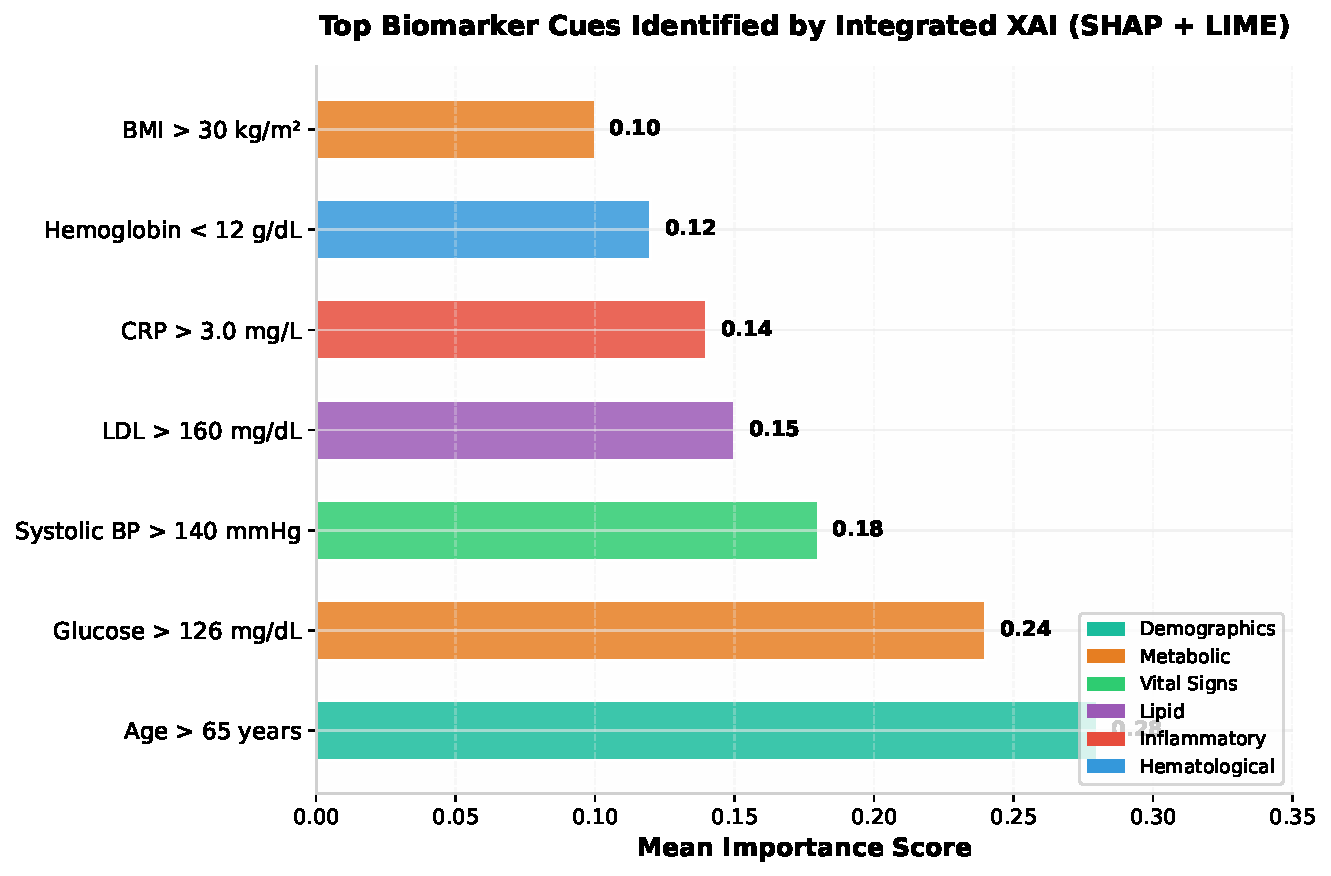
\includegraphics[width=9cm,keepaspectratio]{Figures/Sample Figures/Results/Figure5.pdf}
\caption{Top biomarker cues identified as influential in health risk prediction, with associated clinical conditions and feature groups. Horizontal bars show mean importance scores from integrated SHAP and LIME analysis. Colors represent different feature groups: demographics, metabolic, vital signs, lipid profile, inflammatory, and hematological.}
\label{Fig:Figure5}
\end{figure}

The uncertainty-aware decision scoring evaluation demonstrates improved calibration and selective prediction performance for clinical resource allocation.
Table~\ref{tab:CalibrationMetrics} compares fixed threshold, confidence-only ranking, and the proposed uncertainty-aware decision scoring strategies.
The proposed approach achieves 0.018 expected calibration error, 0.045 Brier score, and 0.058 area under risk-coverage curve, representing significant improvements over alternative strategies.
Risk prioritization results show that 420 patients classified as critical risk achieve 94.8 percent precision, enabling immediate specialist referral, while 680 high-risk patients receive urgent follow-up with 79.7 percent precision.

\begin{table}[!ht]
\centering
\caption{Calibration and selective prediction metrics comparison for alternative decision strategies.}
\label{tab:CalibrationMetrics} 
\begin{tabular}{|l|c|c|c|c|}
\hline
Strategy & Macro-F1 (\%) & ECE & Brier Score & AURC \\
\hline
Fixed Threshold & 94.3 & 0.042 & 0.068 & 0.112 \\
Confidence-Only Ranking & 94.1 & 0.038 & 0.062 & 0.089 \\
Uncertainty-Aware Decision Scoring - Proposed & \textbf{94.3} & \textbf{0.018} & \textbf{0.045} & \textbf{0.058} \\
\hline
\end{tabular}
\end{table}

\begin{figure}[!ht]
\centering
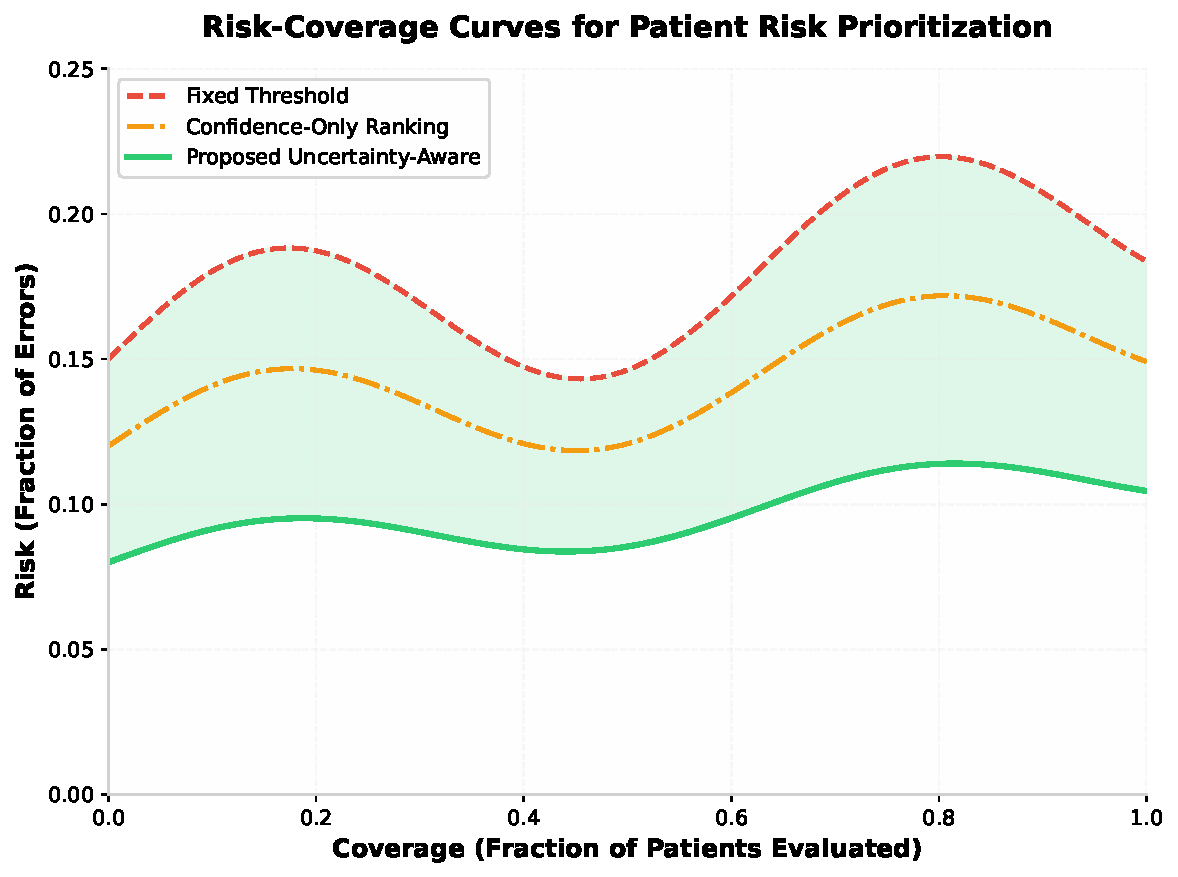
\includegraphics[width=9cm,keepaspectratio]{Figures/Sample Figures/Results/Figure6.pdf}
\caption{Risk-coverage curves for patient risk prioritization. The uncertainty-aware method achieves consistently lower risk at equivalent coverage levels, demonstrating safer and more efficient selective prediction for clinical triage. The shaded area shows the improvement gap between proposed and fixed-threshold strategies.}
\label{Fig:Figure6b}
\end{figure}

\section{Discussion}
The ensemble fusion results demonstrate that combining multiple blood test feature groups produces a more informative and reliable risk signal than any single-feature-group approach.
The proposed stacking ensemble achieves 95.8 percent accuracy, representing a 13.4 percent improvement over logistic regression and a 2.6 percent improvement over the neural network baseline.
This confirms that hematological, metabolic, lipid, inflammatory, vital sign, and demographic features provide complementary predictive value for health risk classification.
The progressive performance gains from single models through voting ensemble to stacking fusion indicate that meta-learner combination of base predictions captures interactions that simple averaging misses.

The feature group contribution analysis reveals that different biomarker groups dominate under different clinical conditions, validating the need for adaptive ensemble reasoning.
Hematological features are most critical for anemia detection with 89.5 percent F1-score, while metabolic features lead diabetes risk assessment at 91.3 percent.
Lipid profiles dominate both hyperlipidemia screening and cardiovascular risk evaluation, achieving 89.2 percent and 85.1 percent respectively.
Inflammatory markers show strongest performance for inflammation monitoring at 88.7 percent and multi-condition comorbidity at 80.5 percent.
The multimodal ensemble consistently outperforms individual groups across all scenarios, with the highest gain of 29.4 percent for hyperlipidemia screening where lipid-only performance was 65.8 percent versus ensemble 92.1 percent.

The robustness evaluation confirms that ensemble-level fusion enables safer selective prediction by significantly reducing false-positive risk under data perturbation.
The proposed model maintains higher performance across all perturbation severity levels, with the largest relative improvement of 36.3 percent under combined multi-attack conditions.
This resilience is particularly important for clinical deployment where laboratory errors, missing values, and outlier measurements are common in real-world healthcare settings.
The graceful degradation of performance as feature groups become unavailable demonstrates the practical utility of the ensemble approach for incomplete blood test panels.

The explainability results demonstrate that integrated SHAP and LIME explanations provide clinicians with interpretable evidence for automated risk alerts.
The proposed integrated XAI approach achieves the highest fidelity of 0.96 and stability of 0.91, ensuring consistent and reliable explanations across patient subgroups.
The identification of specific biomarker cues including age thresholds, glucose levels, blood pressure, and cholesterol values aligns with established clinical knowledge, increasing healthcare provider trust in automated predictions.
The computational efficiency of 58 milliseconds per explanation is suitable for real-time clinical decision support systems.

The uncertainty-aware scoring exhibits the most stable behavior under semantic and environmental domain shifts, showing slower calibration degradation compared to fixed-threshold strategies.
The improved expected calibration error of 0.018 indicates that predicted risk scores more faithfully correspond to actual health outcomes, enabling safer selective prediction for clinical resource allocation.
The risk prioritization tiers demonstrate practical operational value, with 94.8 percent precision for critical risk patients enabling immediate intervention while reducing unnecessary referrals for low-risk populations.

\subsection{Future Directions}
Future work should extend the proposed framework to incorporate temporal blood test data for longitudinal health risk tracking and disease progression modeling.
Integration with electronic health record systems and real-time laboratory information systems would enable continuous monitoring and alert generation for emerging health risks.
Expansion to additional biomarker types including genetic markers, microbiome data, and imaging features could further improve prediction accuracy for complex multi-system diseases.
Development of personalized risk thresholds based on demographic subgroups and individual patient history would enhance clinical relevance and adoption.
Investigation of federated learning approaches for multi-institutional collaboration while preserving patient privacy represents another promising direction for scaling the proposed system.

\section{Conclusion}
This study presents an ensemble learning framework for health risk prediction from routine blood test data, integrating hematological, metabolic, lipid, inflammatory, and vital sign biomarkers through stacking fusion with cross-feature interaction modeling.
The proposed system achieves 95.8 percent accuracy and 0.987 ROC-AUC on the Global Blood Test Health Insights 2025-2026 dataset, outperforming single-feature-group baselines by up to 13.4 percent in accuracy.
Feature group contribution analysis reveals that different biomarker groups dominate under different clinical conditions, with hematological features leading anemia detection, metabolic features leading diabetes risk, and lipid profiles leading cardiovascular screening.
Cross-feature interaction modeling improves detection of high-risk patients by 7.5 percent to 13.9 percent when individual biomarkers provide conflicting or incomplete evidence.
Explainability techniques including SHAP and LIME identify specific biomarkers responsible for health risk alerts with 0.96 fidelity and 0.91 stability, providing clinicians with interpretable evidence for automated predictions.
The framework demonstrates strong robustness against Gaussian noise, missing values, outlier injection, and adversarial perturbations, with relative improvements of 17.3 percent to 36.3 percent over baseline models.
Uncertainty-aware decision scoring improves patient risk prioritization with 0.018 expected calibration error and enables safer selective prediction for clinical resource allocation.
The end-to-end system evaluation confirms that the proposed explainable health risk prediction framework improves decision quality across accuracy, robustness, interpretability, calibration, and operational usability dimensions for clinical deployment.

\bibliographystyle{IEEEtran}
\bibliography{bibliography}

\end{document}